% ---------------------------------------------
\section{Main Idea}
% ---------------------------------------------

Deep learning image classifiers are dominated by two fundamentally different
paradigms: Convolutional Neural Networks (CNNs), which exploit local spatial
structure through learnable filters, and Vision Transformers (ViTs), which model
global patch relationships through self-attention. This miniproject project asks a concrete
question: \textit{given identical training conditions and no pretrained weights,
which architecture learns better representations for a structured, single-domain
image dataset?}

Both models are built from scratch in TensorFlow/Keras and trained on rice grain
images. The comparison isolates architectural design as the sole variable, with
no transfer learning involved.

% ---------------------------------------------
\section{Problem Statement} 
% ---------------------------------------------

The task is a five-class image classification problem. Given a rice grain image,
the model must predict which of five varieties it belongs to: Arborio, Basmati,
Ipsala, Jasmine, or Karacadag. The varieties differ in grain shape, texture, and
size, but are visually similar enough that reliable discrimination requires
learning fine-grained features.

The dataset is the Rice Image Dataset~\cite{rice}, containing 75\,000 JPEG
images ($224\times224$ px), with 15\,000 images per class. Data is split 70/15/15
(train/val/test) using stratified sampling with a fixed seed (42). Training images
receive light augmentation (horizontal flips, $\pm10\%$ rotation, $\pm10\%$ zoom).
Class weights are computed from the training split to handle any residual imbalance.

% ---------------------------------------------
\section{Algorithm}
% ---------------------------------------------

\subsection{CNN}

The CNN is a sequential model with three convolutional blocks followed by a
classification head. Each block applies \texttt{Conv2D} (ReLU) then
\texttt{MaxPooling2D}, doubling filters while halving spatial resolution: 32
filters at $112\times112$, 64 at $56\times56$, and 128 at $28\times28$ with
\texttt{Dropout}($p{=}0.3$). The head flattens the feature map, applies
\texttt{Dense}(128, ReLU) with \texttt{Dropout}($p{=}0.4$), and outputs via
\texttt{Dense}(5, softmax). Total: \textbf{11.2M parameters}.

\subsection{Vision Transformer}

The ViT is implemented from scratch. A \texttt{Conv2D} (kernel 16, stride 16)
embeds each $16\times16$ patch into a 64-d vector, producing a sequence of
$(224/16)^2 = 196$ tokens. Learned positional embeddings are added
element-wise. The sequence is processed by six Transformer encoder blocks,
each with \texttt{LayerNorm} + \texttt{MultiHeadAttention} (4 heads, key dim 64)
and \texttt{LayerNorm} + MLP (128$\to$64, GELU), with Dropout 0.1 throughout.
\texttt{GlobalAveragePooling1D} collapses the sequence, followed by
\texttt{Dropout}(0.1) and \texttt{Dense}(5, softmax).
Total: \textbf{549K parameters} (${\approx}20\times$ fewer than the CNN).

\begin{figure*}[t]
\centering
\begin{minipage}[t]{0.48\textwidth}
  \centering
  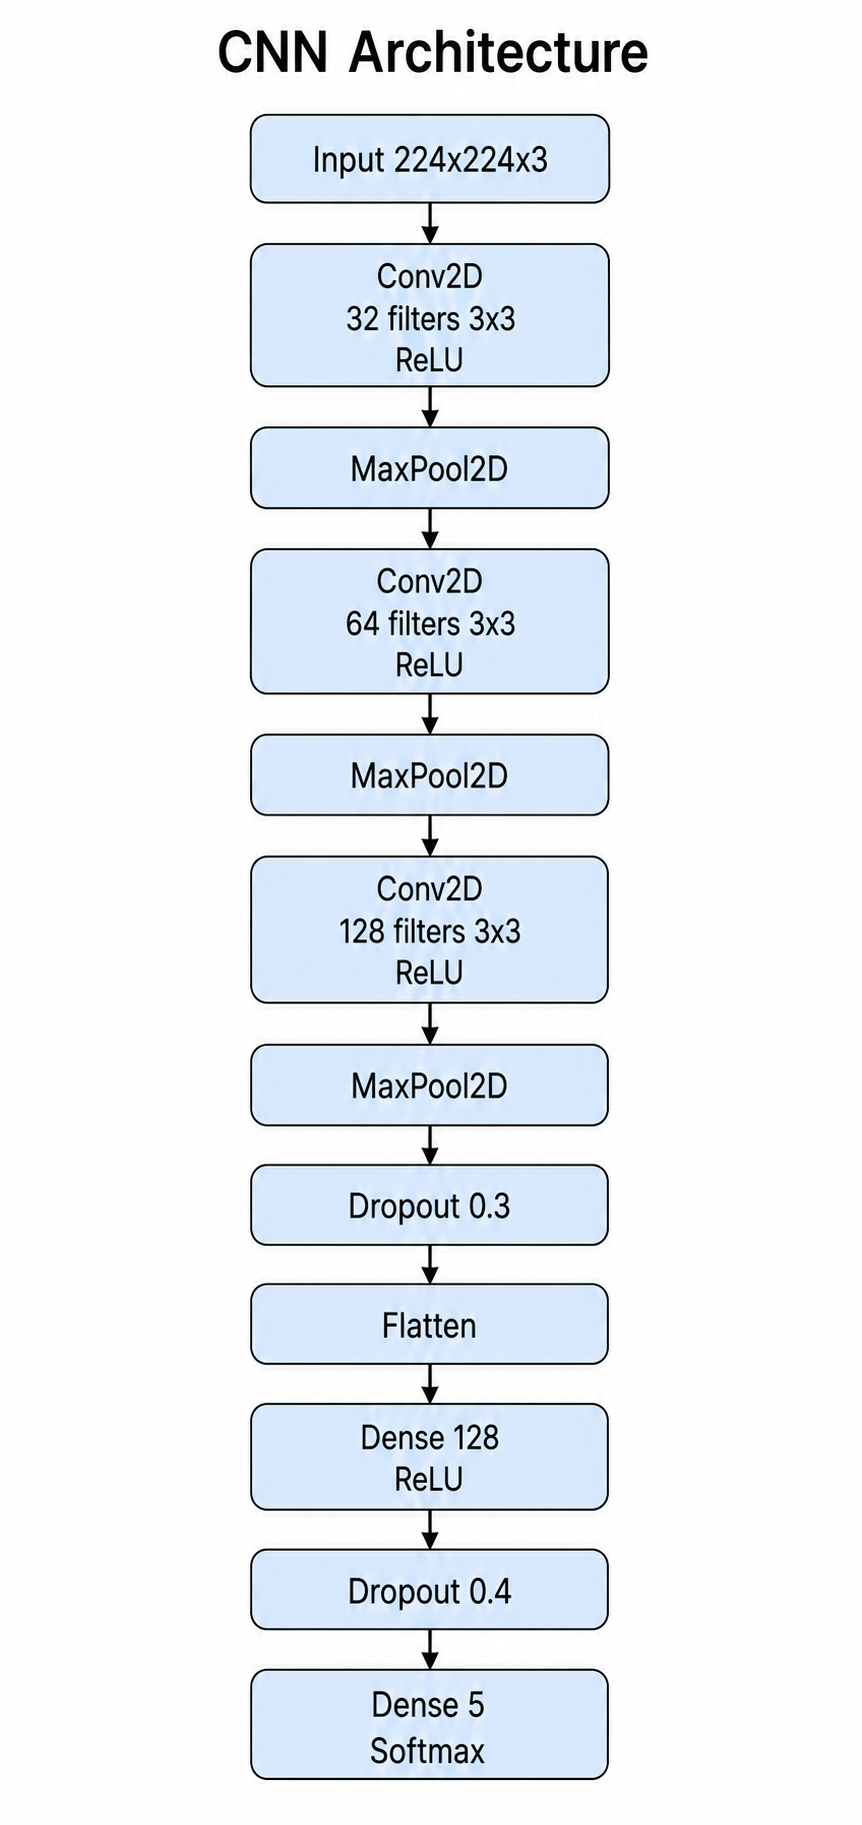
\includegraphics[width=\linewidth]{figures/cnn2.png}
  \caption{CNN architecture overview.}
  \label{fig:cnn}
\end{minipage}
\hfill
\begin{minipage}[t]{0.48\textwidth}
  \centering
  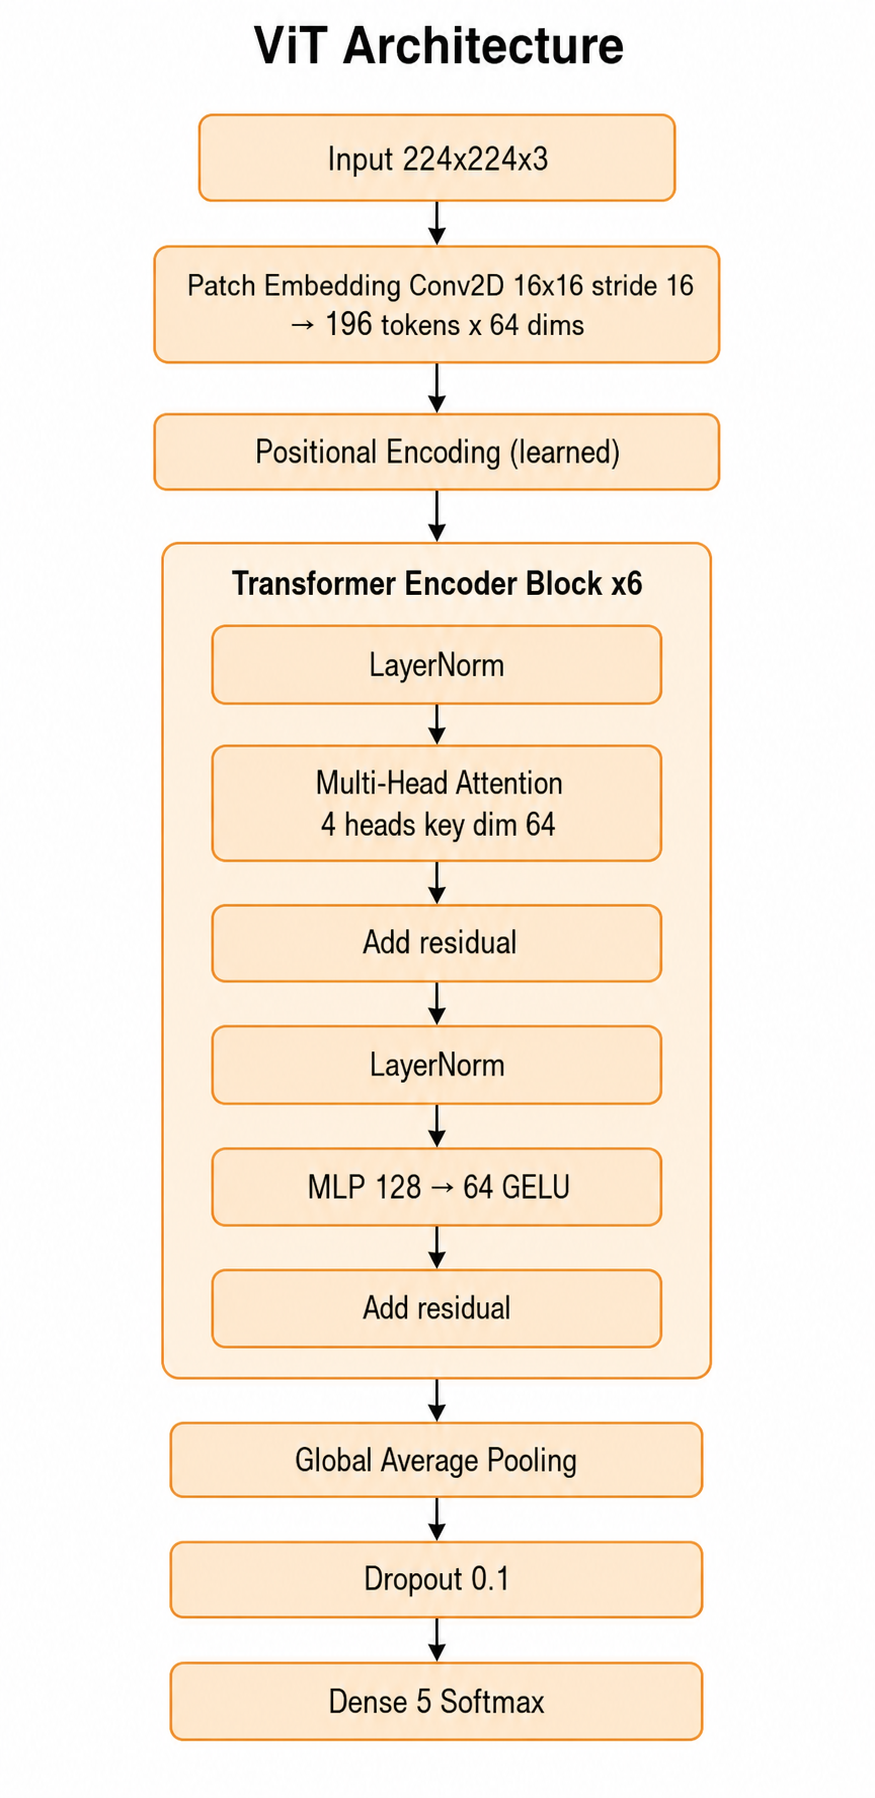
\includegraphics[width=\linewidth]{figures/vit.png}
  \caption{ViT architecture overview.}
  \label{fig:vit}
\end{minipage}
\end{figure*}

\subsection{Training Setup}

Both models share identical training hyperparameters (Table~\ref{tab:hp}).
Adam is used as the optimiser. Three callbacks are active: early stopping
(patience 5, restores best weights), a model checkpoint (saves best validation
model), and learning rate reduction on plateau (ReduceLROnPlateau).
All experiments run in Docker on a dedicated GPU server.

\begin{table}[H]
\centering
\caption{Shared training hyperparameters.}
\label{tab:hp}
\begin{tabular}{@{}ll@{}}
\toprule
\textbf{Hyperparameter}   & \textbf{Value} \\
\midrule
Optimiser                 & Adam \\
Learning rate             & $10^{-3}$ \\
Max epochs                & 20 \\
Batch size                & 32 \\
Early stopping patience   & 5 \\
LR decay factor / patience & 0.5 / 3 \\
Minimum learning rate     & $10^{-6}$ \\
\bottomrule
\end{tabular}
\end{table}

% ---------------------------------------------
\section{Results and Discussion}
% ---------------------------------------------

Table~\ref{tab:results} reports test-set metrics after training. The ViT
outperforms the CNN on both accuracy and loss despite having $20\times$ fewer
parameters, demonstrating that self-attention over patch sequences can capture
discriminative features more compactly than stacked convolutions for this task.

\begin{table}[H]
\centering
\caption{CNN vs.\ ViT on the held-out test set (run \texttt{8f1ed8fb}).}
\label{tab:results}
\begin{tabular}{@{}lrrrr@{}}
\toprule
\textbf{Model} & \textbf{Params} & \textbf{Acc} & \textbf{Loss} & \textbf{Time} \\
\midrule
CNN & 11.2M & 98.71\% & 0.0427 & 351\,s \\
ViT & 0.55M & \textbf{99.49\%} & \textbf{0.0177} & 887\,s \\
\bottomrule
\end{tabular}
\end{table}

Figure~\ref{fig:curves} shows the per-epoch learning curves. The CNN exhibits
intermittent validation-loss spikes at epochs 6--8 and 14 (gap up to $+0.051$),
which ReduceLROnPlateau partially dampens; early stopping triggered at epoch 16.
The ViT converges smoothly, with train and val loss tracking within $\pm0.02$
throughout and reaching its best validation accuracy of \textbf{99.52\%} at
epoch 19.

\begin{figure}[H]
\centering
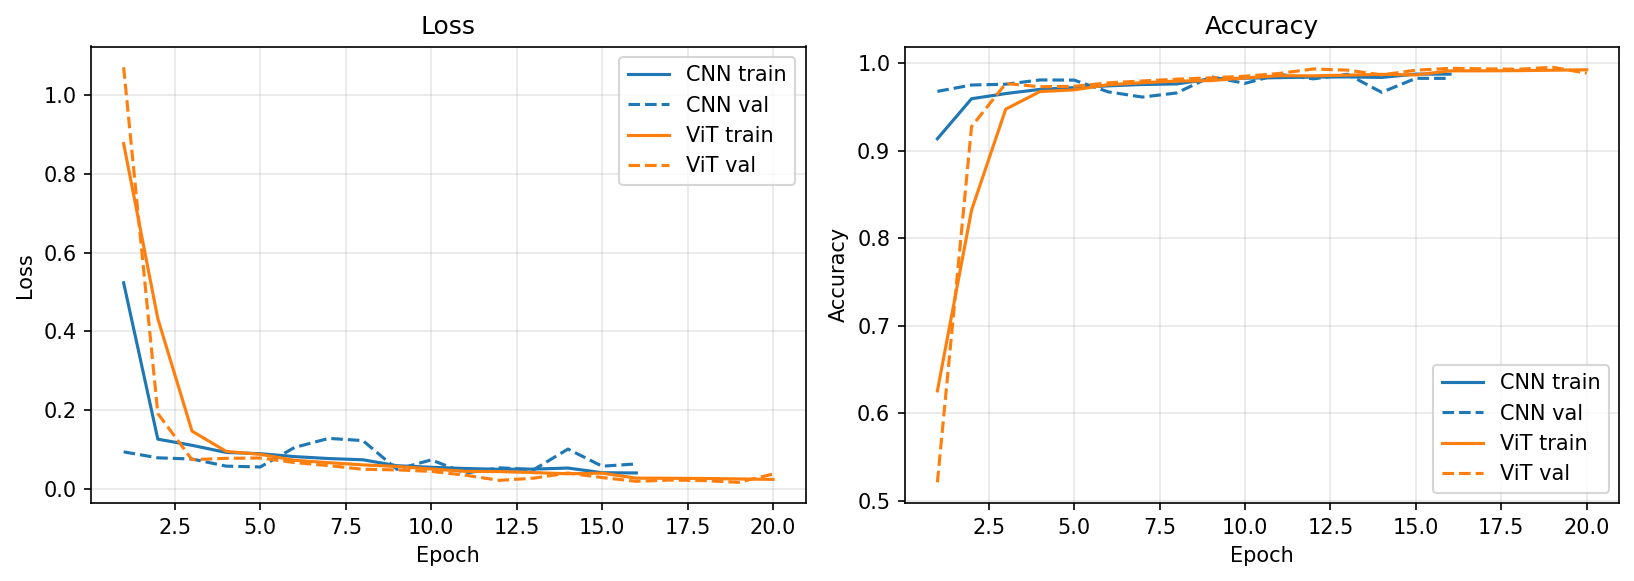
\includegraphics[width=\linewidth]{figures/learning_curves_combined.png}
\caption{Loss (left) and accuracy (right) per epoch. Solid: train; dashed: val.
Blue: CNN; orange: ViT.}
\label{fig:curves}
\end{figure}

Figure~\ref{fig:curves} summarises all four metrics. The ViT advantage is
\textbf{0.78\,pp} in accuracy, translating to roughly 88 fewer misclassifications
on the 11\,250-image test set. Ipsala is the easiest class for both models
(near-perfect F1), likely due to its morphologically distinct round grain shape.
Visually similar long-grain types such as Basmati and Jasmine produce the most
errors. The CNN's instability suggests its feature hierarchy is more sensitive to
the learning-rate schedule; a lower initial lr or stronger weight decay may help.
The ViT's accuracy gain comes at a cost: it trains \textbf{2.5$\times$ slower}
(887\,s vs.\ 351\,s) due to the quadratic attention complexity over 196 patches.

% ---------------------------------------------
\section{Reflection}
% ---------------------------------------------

The most surprising finding is that the ViT outperformed the CNN despite having
far fewer parameters and no pretraining. The conventional wisdom that transformers
require large-scale pretraining to match CNNs on vision tasks did not hold here,
suggesting the rice dataset has enough intra-class regularity for self-attention
to converge from scratch.

The CNN's mid-training instability was unexpected given its stronger spatial
inductive bias. In hindsight, the aggressive initial learning rate ($10^{-3}$)
combined with a relatively small network may have caused the weight updates to
overshoot in the later convolutional blocks, which the LR scheduler only
partially corrected. Future work could address this with a warm-up schedule or
cosine annealing.

A key limitation is that both models are trained on a single, well-curated
dataset with balanced classes and consistent image quality. Generalisation to
noisy real-world data is unknown. Transfer learning from ImageNet would likely
improve both accuracy and training efficiency, and a proper ViT-B/16 baseline
would provide a more meaningful upper bound for the transformer architecture.

\begin{thebibliography}{1}
\bibitem{rice}
M.\ Koklu et al., ``Classification of Rice Varieties with Deep Learning
Methods,'' \textit{Computers and Electronics in Agriculture}, 2021.
\end{thebibliography}

\appendix
\section*{Appendix A: Experimental Platform}

\begin{table}[H]
\centering
\caption{Experimental platform.}
\label{tab:hw}
\begin{tabular}{@{}ll@{}}
\toprule
\textbf{Component} & \textbf{Specification} \\
\midrule
\multicolumn{2}{@{}l}{\textit{Hardware}} \\[2pt]
CPU    & AMD EPYC 9354P, 32 cores / 64 threads \\
Memory & 256\,GB DDR5 \\
GPU    & NVIDIA L40S, 46\,GB GDDR6, PCIe Gen4$\times$16 \\
\midrule
\multicolumn{2}{@{}l}{\textit{Software}} \\[2pt]
OS        & Ubuntu 22.04.5 LTS, kernel 5.15.0-173 \\
CUDA      & 12.6 (V12.6.85) \\
Driver    & 580.95.05 \\
Container & Docker 29.1.3 \\
\bottomrule
\end{tabular}
\end{table}

\section*{Appendix B: Source Code}

The full source code, training scripts, Dockerfile, and results index are
publicly available at:

\begin{center}
\url{https://github.com/entroopie/ai-project-cnn-vs-vit}
\end{center}

\end{document}